\documentclass[twoside]{book}

% Packages required by doxygen
\usepackage{fixltx2e}
\usepackage{calc}
\usepackage{doxygen}
\usepackage[export]{adjustbox} % also loads graphicx
\usepackage{graphicx}
\usepackage[utf8]{inputenc}
\usepackage{makeidx}
\usepackage{multicol}
\usepackage{multirow}
\PassOptionsToPackage{warn}{textcomp}
\usepackage{textcomp}
\usepackage[nointegrals]{wasysym}
\usepackage[table]{xcolor}

% Font selection
\usepackage[T1]{fontenc}
\usepackage[scaled=.90]{helvet}
\usepackage{courier}
\usepackage{amssymb}
\usepackage{sectsty}
\renewcommand{\familydefault}{\sfdefault}
\allsectionsfont{%
  \fontseries{bc}\selectfont%
  \color{darkgray}%
}
\renewcommand{\DoxyLabelFont}{%
  \fontseries{bc}\selectfont%
  \color{darkgray}%
}
\newcommand{\+}{\discretionary{\mbox{\scriptsize$\hookleftarrow$}}{}{}}

% Page & text layout
\usepackage{geometry}
\geometry{%
  a4paper,%
  top=2.5cm,%
  bottom=2.5cm,%
  left=2.5cm,%
  right=2.5cm%
}
\tolerance=750
\hfuzz=15pt
\hbadness=750
\setlength{\emergencystretch}{15pt}
\setlength{\parindent}{0cm}
\setlength{\parskip}{3ex plus 2ex minus 2ex}
\makeatletter
\renewcommand{\paragraph}{%
  \@startsection{paragraph}{4}{0ex}{-1.0ex}{1.0ex}{%
    \normalfont\normalsize\bfseries\SS@parafont%
  }%
}
\renewcommand{\subparagraph}{%
  \@startsection{subparagraph}{5}{0ex}{-1.0ex}{1.0ex}{%
    \normalfont\normalsize\bfseries\SS@subparafont%
  }%
}
\makeatother

% Headers & footers
\usepackage{fancyhdr}
\pagestyle{fancyplain}
\fancyhead[LE]{\fancyplain{}{\bfseries\thepage}}
\fancyhead[CE]{\fancyplain{}{}}
\fancyhead[RE]{\fancyplain{}{\bfseries\leftmark}}
\fancyhead[LO]{\fancyplain{}{\bfseries\rightmark}}
\fancyhead[CO]{\fancyplain{}{}}
\fancyhead[RO]{\fancyplain{}{\bfseries\thepage}}
\fancyfoot[LE]{\fancyplain{}{}}
\fancyfoot[CE]{\fancyplain{}{}}
\fancyfoot[RE]{\fancyplain{}{\bfseries\scriptsize Generated by Doxygen }}
\fancyfoot[LO]{\fancyplain{}{\bfseries\scriptsize Generated by Doxygen }}
\fancyfoot[CO]{\fancyplain{}{}}
\fancyfoot[RO]{\fancyplain{}{}}
\renewcommand{\footrulewidth}{0.4pt}
\renewcommand{\chaptermark}[1]{%
  \markboth{#1}{}%
}
\renewcommand{\sectionmark}[1]{%
  \markright{\thesection\ #1}%
}

% Indices & bibliography
\usepackage{natbib}
\usepackage[titles]{tocloft}
\setcounter{tocdepth}{3}
\setcounter{secnumdepth}{5}
\makeindex

% Hyperlinks (required, but should be loaded last)
\usepackage{ifpdf}
\ifpdf
  \usepackage[pdftex,pagebackref=true]{hyperref}
\else
  \usepackage[ps2pdf,pagebackref=true]{hyperref}
\fi
\hypersetup{%
  colorlinks=true,%
  linkcolor=blue,%
  citecolor=blue,%
  unicode%
}

% Custom commands
\newcommand{\clearemptydoublepage}{%
  \newpage{\pagestyle{empty}\cleardoublepage}%
}

\usepackage{caption}
\captionsetup{labelsep=space,justification=centering,font={bf},singlelinecheck=off,skip=4pt,position=top}

%===== C O N T E N T S =====

\begin{document}

% Titlepage & ToC
\hypersetup{pageanchor=false,
             bookmarksnumbered=true,
             pdfencoding=unicode
            }
\pagenumbering{roman}
\begin{titlepage}
\vspace*{7cm}
\begin{center}%
{\Large npc-\/game }\\
\vspace*{1cm}
{\large Generated by Doxygen 1.8.11}\\
\end{center}
\end{titlepage}
\clearemptydoublepage
\tableofcontents
\clearemptydoublepage
\pagenumbering{arabic}
\hypersetup{pageanchor=true}

%--- Begin generated contents ---
\chapter{npc-\/game}
\label{md_README}
\hypertarget{md_README}{}
Final Fantasy-\/style Role-\/\+Playing Game about the non-\/heroic non-\/player characters inhabiting the world in a traditional example of such a game. Multiplatform via Simple Directmedia Layer (S\+D\+L2) C++ Library. Also uses Boost.

Requires the following libraries\+: S\+D\+L2 (\href{https://www.libsdl.org/download-2.0.php}{\tt https\+://www.\+libsdl.\+org/download-\/2.\+0.\+php}) S\+D\+L2\+\_\+\+Image (\href{https://www.libsdl.org/projects/SDL_image/}{\tt https\+://www.\+libsdl.\+org/projects/\+S\+D\+L\+\_\+image/}) S\+D\+L2\+\_\+ttf (\href{https://www.libsdl.org/projects/SDL_ttf/}{\tt https\+://www.\+libsdl.\+org/projects/\+S\+D\+L\+\_\+ttf/}) Boost (\href{http://sourceforge.net/projects/boost/files/latest/download?source=files}{\tt http\+://sourceforge.\+net/projects/boost/files/latest/download?source=files})

Code by Samuel Weber (sbweber). npc-\/game.\+rar contains a playable, self-\/contained, current Windows release build of the game.

Default Controls\+: Arrow keys\+: Move around the map. z\+: Interact with things on the map. esc\+: Go back/up a layer. Currently unused. f4\+: Quit the program from anywhere. F12\+: Go to the title screen. Click on a tile on the map to move to it. Click on a sprite to interact with it. To advance text, press any key or click anywhere in the window.

Debug Controls\+: 1\+: Load map \char`\"{}0,0.\+txt\char`\"{}. 2\+: Load map \char`\"{}0,1.\+txt\char`\"{}. 9\+: Go to the key rebind menu. f\+: Go to the test case for battles. Currently locks you into the battle state with no way out except the debug controls.

Explanation of Licenses\+: L\+I\+C\+E\+N\+SE is the (M\+IT) license for this project itself. L\+I\+C\+E\+N\+S\+E-\/\+S\+D\+L2 is the (zlib) license for the S\+D\+L2 library. L\+I\+C\+E\+N\+S\+E.\+md is the (M\+IT) license for the Find\+S\+D\+L2$\ast$.cmake files, the C\+Make\+Lists.\+txt (further modified from its original version), and some scattered code throughout the project (this project began its life by following the Twinklebear\+Dev S\+DL 2.\+0 Lessons, from here \href{https://github.com/Twinklebear/TwinklebearDev-Lessons}{\tt https\+://github.\+com/\+Twinklebear/\+Twinklebear\+Dev-\/\+Lessons}). Copyright.\+txt is the (B\+SD 3-\/clause) license for the Boost libraries. 
\chapter{Hierarchical Index}
\section{Class Hierarchy}
This inheritance list is sorted roughly, but not completely, alphabetically\+:\begin{DoxyCompactList}
\item \contentsline{section}{Button}{\pageref{class_button}}{}
\item \contentsline{section}{Party}{\pageref{class_party}}{}
\item \contentsline{section}{Sprite}{\pageref{class_sprite}}{}
\item \contentsline{section}{Terr}{\pageref{class_terr}}{}
\item \contentsline{section}{Tile}{\pageref{class_tile}}{}
\begin{DoxyCompactList}
\item \contentsline{section}{Warp}{\pageref{class_warp}}{}
\end{DoxyCompactList}
\item \contentsline{section}{Unit}{\pageref{class_unit}}{}
\end{DoxyCompactList}

\chapter{Class Index}
\section{Class List}
Here are the classes, structs, unions and interfaces with brief descriptions\+:\begin{DoxyCompactList}
\item\contentsline{section}{\hyperlink{class_button}{Button} \\*Describes a clickable button }{\pageref{class_button}}{}
\item\contentsline{section}{\hyperlink{class_party}{Party} }{\pageref{class_party}}{}
\item\contentsline{section}{\hyperlink{class_sprite}{Sprite} \\*Visual half of a \hyperlink{class_unit}{Unit}. Information on what to draw to put a sprite onscreen }{\pageref{class_sprite}}{}
\item\contentsline{section}{\hyperlink{class_terr}{Terr} \\*Describes an overworld map. All maps currently must be rectangles }{\pageref{class_terr}}{}
\item\contentsline{section}{\hyperlink{class_tile}{Tile} \\*Data about individual tiles from a \hyperlink{class_terr}{Terr} }{\pageref{class_tile}}{}
\item\contentsline{section}{\hyperlink{class_unit}{Unit} \\*Backend of a character’s data. Visual depiction handled by \hyperlink{class_sprite}{Sprite} class }{\pageref{class_unit}}{}
\item\contentsline{section}{\hyperlink{class_warp}{Warp} \\*\hyperlink{class_warp}{Warp} is a kind of \hyperlink{class_tile}{Tile} that loads a new \hyperlink{class_terr}{Terr} (e.\+g. leaving a building) }{\pageref{class_warp}}{}
\end{DoxyCompactList}

\chapter{Class Documentation}
\hypertarget{class_attack}{}\section{Attack Class Reference}
\label{class_attack}\index{Attack@{Attack}}


Data for an attack. Damage amount, type, and accuracy.  




{\ttfamily \#include $<$Attack.\+h$>$}

\subsection*{Public Member Functions}
\begin{DoxyCompactItemize}
\item 
\hyperlink{class_attack_ae96e4933fd3b60a53543491d15f05913}{Attack} (long dam, long a, damage\+Type e)\hypertarget{class_attack_ae96e4933fd3b60a53543491d15f05913}{}\label{class_attack_ae96e4933fd3b60a53543491d15f05913}

\begin{DoxyCompactList}\small\item\em \hyperlink{class_attack}{Attack} constructor. \end{DoxyCompactList}\item 
long \hyperlink{class_attack_a2212805bb57a3da698bf720b213c5304}{get\+Acc} ()\hypertarget{class_attack_a2212805bb57a3da698bf720b213c5304}{}\label{class_attack_a2212805bb57a3da698bf720b213c5304}

\begin{DoxyCompactList}\small\item\em Returns accuracy of attack. \end{DoxyCompactList}\item 
long \hyperlink{class_attack_ad2826485a531b1b885a0ed6618b175da}{get\+Damage} ()\hypertarget{class_attack_ad2826485a531b1b885a0ed6618b175da}{}\label{class_attack_ad2826485a531b1b885a0ed6618b175da}

\begin{DoxyCompactList}\small\item\em Returns base damage of attack. \end{DoxyCompactList}\item 
damage\+Type \hyperlink{class_attack_af9a766300c7ae142bb29bb47f421e281}{get\+Element} ()\hypertarget{class_attack_af9a766300c7ae142bb29bb47f421e281}{}\label{class_attack_af9a766300c7ae142bb29bb47f421e281}

\begin{DoxyCompactList}\small\item\em Returns element of attack. \end{DoxyCompactList}\end{DoxyCompactItemize}
\subsection*{Protected Attributes}
\begin{DoxyCompactItemize}
\item 
long \hyperlink{class_attack_adabef93e40cf94f3dac58532b3fddac2}{damage}\hypertarget{class_attack_adabef93e40cf94f3dac58532b3fddac2}{}\label{class_attack_adabef93e40cf94f3dac58532b3fddac2}

\begin{DoxyCompactList}\small\item\em \hyperlink{class_attack}{Attack}\textquotesingle{}s base damage. \end{DoxyCompactList}\item 
long \hyperlink{class_attack_aa109887bd6e479de6c01bb6fd3128e10}{acc}\hypertarget{class_attack_aa109887bd6e479de6c01bb6fd3128e10}{}\label{class_attack_aa109887bd6e479de6c01bb6fd3128e10}

\begin{DoxyCompactList}\small\item\em \hyperlink{class_attack}{Attack}\textquotesingle{}s accuracy. \end{DoxyCompactList}\item 
damage\+Type \hyperlink{class_attack_a0910777fac28d0a017e5ab7d976984fb}{element}\hypertarget{class_attack_a0910777fac28d0a017e5ab7d976984fb}{}\label{class_attack_a0910777fac28d0a017e5ab7d976984fb}

\begin{DoxyCompactList}\small\item\em Element of attack. \end{DoxyCompactList}\end{DoxyCompactItemize}


\subsection{Detailed Description}
Data for an attack. Damage amount, type, and accuracy. 

The documentation for this class was generated from the following files\+:\begin{DoxyCompactItemize}
\item 
Attack.\+h\item 
Attack.\+cpp\end{DoxyCompactItemize}

\hypertarget{class_button}{}\section{Button Class Reference}
\label{class_button}\index{Button@{Button}}


Describes a clickable button.  




{\ttfamily \#include $<$Button.\+h$>$}

\subsection*{Public Member Functions}
\begin{DoxyCompactItemize}
\item 
\hyperlink{class_button_a605828617975a0a3a330dbebbfa736bf}{Button} (S\+D\+L\+\_\+\+Renderer $\ast$ren, const string \&file, int x, int y, int w, int h, T\+T\+F\+\_\+\+Font $\ast$font=nullptr, const string \&s=\char`\"{}\char`\"{})
\item 
bool \hyperlink{class_button_a1f93070fbcb76faac1b26df1cf04a9e4}{button\+Click} (S\+D\+L\+\_\+\+Renderer $\ast$ren, S\+D\+L\+\_\+\+Mouse\+Button\+Event \&click)\hypertarget{class_button_a1f93070fbcb76faac1b26df1cf04a9e4}{}\label{class_button_a1f93070fbcb76faac1b26df1cf04a9e4}

\begin{DoxyCompactList}\small\item\em Returns true if \hyperlink{class_button}{Button} was clicked. \end{DoxyCompactList}\item 
S\+D\+L\+\_\+\+Rect \hyperlink{class_button_a4aa8e2b4fdc41c911ce7ebbe04ba27f8}{get\+Pos} ()\hypertarget{class_button_a4aa8e2b4fdc41c911ce7ebbe04ba27f8}{}\label{class_button_a4aa8e2b4fdc41c911ce7ebbe04ba27f8}

\begin{DoxyCompactList}\small\item\em Returns button. \end{DoxyCompactList}\item 
bool \hyperlink{class_button_aecc3cba90d8121c6f673b600c13e4bc9}{mouse\+On\+Button} (int x, int y)\hypertarget{class_button_aecc3cba90d8121c6f673b600c13e4bc9}{}\label{class_button_aecc3cba90d8121c6f673b600c13e4bc9}

\begin{DoxyCompactList}\small\item\em Returns true if mouse is over the button (x/y coords). \end{DoxyCompactList}\item 
bool \hyperlink{class_button_a92f3a17475a7a06b82779b1092a1952f}{mouse\+On\+Button} (S\+D\+L\+\_\+\+Mouse\+Button\+Event \&mouse)\hypertarget{class_button_a92f3a17475a7a06b82779b1092a1952f}{}\label{class_button_a92f3a17475a7a06b82779b1092a1952f}

\begin{DoxyCompactList}\small\item\em Returns true if mouse is over the button (click). \end{DoxyCompactList}\item 
bool \hyperlink{class_button_a2b3d75341a6cc59a0a50730a977cd104}{mouse\+On\+Button} (S\+D\+L\+\_\+\+Mouse\+Motion\+Event \&mouse)\hypertarget{class_button_a2b3d75341a6cc59a0a50730a977cd104}{}\label{class_button_a2b3d75341a6cc59a0a50730a977cd104}

\begin{DoxyCompactList}\small\item\em Returns true if mouse is over the button (mouseover). \end{DoxyCompactList}\item 
void \hyperlink{class_button_a8afc12afd3beb237b7c17e7d00ce3a95}{render} (S\+D\+L\+\_\+\+Renderer $\ast$ren, button\+State state)\hypertarget{class_button_a8afc12afd3beb237b7c17e7d00ce3a95}{}\label{class_button_a8afc12afd3beb237b7c17e7d00ce3a95}

\begin{DoxyCompactList}\small\item\em Draws \hyperlink{class_button}{Button} on the renderer. \end{DoxyCompactList}\end{DoxyCompactItemize}
\subsection*{Protected Attributes}
\begin{DoxyCompactItemize}
\item 
S\+D\+L\+\_\+\+Rect \hyperlink{class_button_aa552275b84734a66578ab684e51ab64a}{button}\hypertarget{class_button_aa552275b84734a66578ab684e51ab64a}{}\label{class_button_aa552275b84734a66578ab684e51ab64a}

\begin{DoxyCompactList}\small\item\em Rectangle describing \hyperlink{class_button}{Button}\textquotesingle{}s position and dimensions. \end{DoxyCompactList}\item 
S\+D\+L\+\_\+\+Texture $\ast$ \hyperlink{class_button_adf19f779ff118533b103aedcf743b8bf}{pic}\hypertarget{class_button_adf19f779ff118533b103aedcf743b8bf}{}\label{class_button_adf19f779ff118533b103aedcf743b8bf}

\begin{DoxyCompactList}\small\item\em \hyperlink{class_button}{Button}\textquotesingle{}s background picture. \end{DoxyCompactList}\item 
S\+D\+L\+\_\+\+Texture $\ast$ \hyperlink{class_button_a08d8969454e7a566717d2488a788bd78}{text}\hypertarget{class_button_a08d8969454e7a566717d2488a788bd78}{}\label{class_button_a08d8969454e7a566717d2488a788bd78}

\begin{DoxyCompactList}\small\item\em \hyperlink{class_button}{Button}\textquotesingle{}s optional foreground text, as a texture. \end{DoxyCompactList}\end{DoxyCompactItemize}


\subsection{Detailed Description}
Describes a clickable button. 

\subsection{Constructor \& Destructor Documentation}
\index{Button@{Button}!Button@{Button}}
\index{Button@{Button}!Button@{Button}}
\subsubsection[{\texorpdfstring{Button(\+S\+D\+L\+\_\+\+Renderer $\ast$ren, const string \&file, int x, int y, int w, int h, T\+T\+F\+\_\+\+Font $\ast$font=nullptr, const string \&s="""")}{Button(SDL_Renderer *ren, const string &file, int x, int y, int w, int h, TTF_Font *font=nullptr, const string &s="")}}]{\setlength{\rightskip}{0pt plus 5cm}Button\+::\+Button (
\begin{DoxyParamCaption}
\item[{S\+D\+L\+\_\+\+Renderer $\ast$}]{ren, }
\item[{const string \&}]{file, }
\item[{int}]{x, }
\item[{int}]{y, }
\item[{int}]{w, }
\item[{int}]{h, }
\item[{T\+T\+F\+\_\+\+Font $\ast$}]{font = {\ttfamily nullptr}, }
\item[{const string \&}]{s = {\ttfamily \char`\"{}\char`\"{}}}
\end{DoxyParamCaption}
)}\hypertarget{class_button_a605828617975a0a3a330dbebbfa736bf}{}\label{class_button_a605828617975a0a3a330dbebbfa736bf}
\hyperlink{class_button}{Button} does not have a default constructor. A \hyperlink{class_button}{Button} must have a position and dimensions, and the constructor requires a filename for the background pic. Text and font are optional. 

The documentation for this class was generated from the following files\+:\begin{DoxyCompactItemize}
\item 
Button.\+h\item 
Button.\+cpp\end{DoxyCompactItemize}

\hypertarget{class_game_state}{}\section{Game\+State Class Reference}
\label{class_game_state}\index{Game\+State@{Game\+State}}


The game\textquotesingle{}s current state. Handles the main event loop.  




{\ttfamily \#include $<$Game\+State.\+h$>$}

\subsection*{Public Member Functions}
\begin{DoxyCompactItemize}
\item 
\hyperlink{class_game_state_a6075ad239ad5e9cbb08da3e7b97fe676}{Game\+State} (S\+D\+L\+\_\+\+Renderer $\ast$ren, T\+T\+F\+\_\+\+Font $\ast$f)\hypertarget{class_game_state_a6075ad239ad5e9cbb08da3e7b97fe676}{}\label{class_game_state_a6075ad239ad5e9cbb08da3e7b97fe676}

\begin{DoxyCompactList}\small\item\em \hyperlink{class_game_state}{Game\+State} constructor. \end{DoxyCompactList}\item 
\hyperlink{class_game_state_ae623df5042cd0c17daa3394fdcb397b3}{$\sim$\+Game\+State} ()\hypertarget{class_game_state_ae623df5042cd0c17daa3394fdcb397b3}{}\label{class_game_state_ae623df5042cd0c17daa3394fdcb397b3}

\begin{DoxyCompactList}\small\item\em \hyperlink{class_game_state}{Game\+State} destructor. \end{DoxyCompactList}\item 
void \hyperlink{class_game_state_a6635a5af1ea4211afcfec058445ff933}{advance} (S\+D\+L\+\_\+\+Event \&e)\hypertarget{class_game_state_a6635a5af1ea4211afcfec058445ff933}{}\label{class_game_state_a6635a5af1ea4211afcfec058445ff933}

\begin{DoxyCompactList}\small\item\em Loop to select which event loop to run. Advances state. \end{DoxyCompactList}\item 
void \hyperlink{class_game_state_ab3c0c9f3f38b875735cfe39ce6a2c154}{change\+Terr} (const string \&new\+Terr)\hypertarget{class_game_state_ab3c0c9f3f38b875735cfe39ce6a2c154}{}\label{class_game_state_ab3c0c9f3f38b875735cfe39ce6a2c154}

\begin{DoxyCompactList}\small\item\em Changes the active \hyperlink{class_terr}{Terr}. \end{DoxyCompactList}\item 
void \hyperlink{class_game_state_ab0ecc413fbf4772869e037bc3489f26e}{dec\+Cursor\+Pos} (unsigned int max)\hypertarget{class_game_state_ab0ecc413fbf4772869e037bc3489f26e}{}\label{class_game_state_ab0ecc413fbf4772869e037bc3489f26e}

\begin{DoxyCompactList}\small\item\em subtracts one from cursor\+Pos, looping to max if needed. \end{DoxyCompactList}\item 
void \hyperlink{class_game_state_a1f40f501f25ae4ea245a6e3011ac85fd}{inc\+Cursor\+Pos} (unsigned int max)\hypertarget{class_game_state_a1f40f501f25ae4ea245a6e3011ac85fd}{}\label{class_game_state_a1f40f501f25ae4ea245a6e3011ac85fd}

\begin{DoxyCompactList}\small\item\em Adds one to cursor\+Pos, looping to zero if needed. \end{DoxyCompactList}\item 
long \hyperlink{class_game_state_a64caafde825c0fc890e41d24d12c3927}{rng} (long min, long max)\hypertarget{class_game_state_a64caafde825c0fc890e41d24d12c3927}{}\label{class_game_state_a64caafde825c0fc890e41d24d12c3927}

\begin{DoxyCompactList}\small\item\em Returns a uniformly distributed random number between min and max. \end{DoxyCompactList}\item 
void \hyperlink{class_game_state_af81371645645ecd84d5d2a246e97d14d}{set\+State} (game\+State gs)\hypertarget{class_game_state_af81371645645ecd84d5d2a246e97d14d}{}\label{class_game_state_af81371645645ecd84d5d2a246e97d14d}

\begin{DoxyCompactList}\small\item\em Sets game\+State. \end{DoxyCompactList}\item 
shared\+\_\+ptr$<$ \hyperlink{class_tile}{Tile} $>$ \hyperlink{class_game_state_a12e67e467e0c1be59d5b681b95e33120}{tile\+Click} (S\+D\+L\+\_\+\+Mouse\+Button\+Event \&click)\hypertarget{class_game_state_a12e67e467e0c1be59d5b681b95e33120}{}\label{class_game_state_a12e67e467e0c1be59d5b681b95e33120}

\begin{DoxyCompactList}\small\item\em Used when clicking on the map. Returns a pointer to the \hyperlink{class_tile}{Tile} clicked. \end{DoxyCompactList}\end{DoxyCompactItemize}
\subsection*{Protected Member Functions}
\begin{DoxyCompactItemize}
\item 
void \hyperlink{class_game_state_ad80bf372b6f644a79b31e97fc4b61532}{interact\+Message\+Handler} (string \&message)\hypertarget{class_game_state_ad80bf372b6f644a79b31e97fc4b61532}{}\label{class_game_state_ad80bf372b6f644a79b31e97fc4b61532}

\begin{DoxyCompactList}\small\item\em Message handler for sprites interacting. \end{DoxyCompactList}\item 
void \hyperlink{class_game_state_a6bcac85dc5a7ce95e58c32d0948b54df}{loop\+Any\+State} (S\+D\+L\+\_\+\+Event \&e)\hypertarget{class_game_state_a6bcac85dc5a7ce95e58c32d0948b54df}{}\label{class_game_state_a6bcac85dc5a7ce95e58c32d0948b54df}

\begin{DoxyCompactList}\small\item\em Loop to handle input that’s treated the same in all states. \end{DoxyCompactList}\item 
void \hyperlink{class_game_state_a78ccdca45d646c8bec157fb6207ada04}{loop\+Battle} (S\+D\+L\+\_\+\+Event \&e)\hypertarget{class_game_state_a78ccdca45d646c8bec157fb6207ada04}{}\label{class_game_state_a78ccdca45d646c8bec157fb6207ada04}

\begin{DoxyCompactList}\small\item\em Loop to process actions in battle state. \end{DoxyCompactList}\item 
void \hyperlink{class_game_state_a8eababbfcac6ae424541fb61e8534682}{loop\+Battle\+Fight} ()\hypertarget{class_game_state_a8eababbfcac6ae424541fb61e8534682}{}\label{class_game_state_a8eababbfcac6ae424541fb61e8534682}

\begin{DoxyCompactList}\small\item\em Subloop for the \textquotesingle{}fight\textquotesingle{} command in battle. \end{DoxyCompactList}\item 
void \hyperlink{class_game_state_ac3101f8eba8251f27acfcf082140908d}{loop\+Battle\+Run} ()\hypertarget{class_game_state_ac3101f8eba8251f27acfcf082140908d}{}\label{class_game_state_ac3101f8eba8251f27acfcf082140908d}

\begin{DoxyCompactList}\small\item\em Subloop for the \textquotesingle{}run\textquotesingle{} command in battle. \end{DoxyCompactList}\item 
void \hyperlink{class_game_state_a87291e60906c205c34fa84ea957fa898}{loop\+Map} (S\+D\+L\+\_\+\+Event \&e)\hypertarget{class_game_state_a87291e60906c205c34fa84ea957fa898}{}\label{class_game_state_a87291e60906c205c34fa84ea957fa898}

\begin{DoxyCompactList}\small\item\em Loop to process inputs while on overworld map. \end{DoxyCompactList}\item 
void \hyperlink{class_game_state_abd3d3df0598dd6731117cab805fa0eef}{loop\+Rebind} (S\+D\+L\+\_\+\+Event \&e)\hypertarget{class_game_state_abd3d3df0598dd6731117cab805fa0eef}{}\label{class_game_state_abd3d3df0598dd6731117cab805fa0eef}

\begin{DoxyCompactList}\small\item\em Loop to process inputs and events while in the key binding menu. \end{DoxyCompactList}\item 
void \hyperlink{class_game_state_a1fff6670e9d9ce3806d7261cfd829237}{loop\+Title} (S\+D\+L\+\_\+\+Event \&e)\hypertarget{class_game_state_a1fff6670e9d9ce3806d7261cfd829237}{}\label{class_game_state_a1fff6670e9d9ce3806d7261cfd829237}

\begin{DoxyCompactList}\small\item\em Loop to process inputs on the title screen. \end{DoxyCompactList}\end{DoxyCompactItemize}
\subsection*{Protected Attributes}
\begin{DoxyCompactItemize}
\item 
unsigned int \hyperlink{class_game_state_a31555272335ffcfb24af67bc826e1521}{cursor\+Pos}\hypertarget{class_game_state_a31555272335ffcfb24af67bc826e1521}{}\label{class_game_state_a31555272335ffcfb24af67bc826e1521}

\begin{DoxyCompactList}\small\item\em Position of cursor in menus. \end{DoxyCompactList}\item 
vector$<$ shared\+\_\+ptr$<$ \hyperlink{class_unit}{Unit} $>$ $>$ \hyperlink{class_game_state_a5a075a4ab1460fb1035c6b87c56e6c05}{enemies}\hypertarget{class_game_state_a5a075a4ab1460fb1035c6b87c56e6c05}{}\label{class_game_state_a5a075a4ab1460fb1035c6b87c56e6c05}

\begin{DoxyCompactList}\small\item\em Vector of enemy units for battle. \end{DoxyCompactList}\item 
T\+T\+F\+\_\+\+Font $\ast$ \hyperlink{class_game_state_a39f32585535aa7a90c2e66f1e6d474e0}{font}\hypertarget{class_game_state_a39f32585535aa7a90c2e66f1e6d474e0}{}\label{class_game_state_a39f32585535aa7a90c2e66f1e6d474e0}

\begin{DoxyCompactList}\small\item\em Primary font for regular usage. \end{DoxyCompactList}\item 
mt19937\+\_\+64 \hyperlink{class_game_state_a64e33a5deae96a673585c1a408abce5a}{rand\+Num\+Gen}\hypertarget{class_game_state_a64e33a5deae96a673585c1a408abce5a}{}\label{class_game_state_a64e33a5deae96a673585c1a408abce5a}

\begin{DoxyCompactList}\small\item\em Random Number Generator. \end{DoxyCompactList}\item 
unique\+\_\+ptr$<$ \hyperlink{class_party}{Party} $>$ \hyperlink{class_game_state_a90d33253ae1bf970ec7f89b2f3975048}{party}\hypertarget{class_game_state_a90d33253ae1bf970ec7f89b2f3975048}{}\label{class_game_state_a90d33253ae1bf970ec7f89b2f3975048}

\begin{DoxyCompactList}\small\item\em The player\textquotesingle{}s party. \end{DoxyCompactList}\item 
game\+State \hyperlink{class_game_state_a90969808e5db25eb4f0ae6b7be027c65}{state}\hypertarget{class_game_state_a90969808e5db25eb4f0ae6b7be027c65}{}\label{class_game_state_a90969808e5db25eb4f0ae6b7be027c65}

\begin{DoxyCompactList}\small\item\em State of game. \end{DoxyCompactList}\item 
unique\+\_\+ptr$<$ \hyperlink{class_terr}{Terr} $>$ \hyperlink{class_game_state_ae2450c36c6b73d979978b22523f3521c}{terr}\hypertarget{class_game_state_ae2450c36c6b73d979978b22523f3521c}{}\label{class_game_state_ae2450c36c6b73d979978b22523f3521c}

\begin{DoxyCompactList}\small\item\em Currently loaded terr. \end{DoxyCompactList}\item 
S\+D\+L\+\_\+\+Timer\+ID \hyperlink{class_game_state_a69d14a618108634864b0b547a5e1b5c5}{timer\+ID}\hypertarget{class_game_state_a69d14a618108634864b0b547a5e1b5c5}{}\label{class_game_state_a69d14a618108634864b0b547a5e1b5c5}

\begin{DoxyCompactList}\small\item\em Timer for regular events. \end{DoxyCompactList}\end{DoxyCompactItemize}


\subsection{Detailed Description}
The game\textquotesingle{}s current state. Handles the main event loop. 

The documentation for this class was generated from the following files\+:\begin{DoxyCompactItemize}
\item 
Game\+State.\+h\item 
Game\+State.\+cpp\end{DoxyCompactItemize}

\hypertarget{class_party}{}\section{Party Class Reference}
\label{class_party}\index{Party@{Party}}
\subsection*{Public Member Functions}
\begin{DoxyCompactItemize}
\item 
{\bfseries Party} (S\+D\+L\+\_\+\+Renderer $\ast$ren)\hypertarget{class_party_a950ef19c74b4ff434064d909145b4190}{}\label{class_party_a950ef19c74b4ff434064d909145b4190}

\item 
\hyperlink{class_sprite}{Sprite} $\ast$ {\bfseries get\+Sprite} ()\hypertarget{class_party_a79d7e55a83b66a41146679deb3b4c533}{}\label{class_party_a79d7e55a83b66a41146679deb3b4c533}

\item 
void {\bfseries set\+Sprite} (S\+D\+L\+\_\+\+Renderer $\ast$ren, const string \&str)\hypertarget{class_party_abe069ffbbf3352f6b39246c8382dd26b}{}\label{class_party_abe069ffbbf3352f6b39246c8382dd26b}

\end{DoxyCompactItemize}
\subsection*{Protected Attributes}
\begin{DoxyCompactItemize}
\item 
\hyperlink{class_unit}{Unit} $\ast$ {\bfseries active} \mbox{[}4\mbox{]}\hypertarget{class_party_aca0245ec21a99d76c4f1d00b7299629a}{}\label{class_party_aca0245ec21a99d76c4f1d00b7299629a}

\item 
vector$<$ \hyperlink{class_unit}{Unit} $\ast$ $>$ {\bfseries passive}\hypertarget{class_party_ab1e00e761df6f415ed72a920d4aa9ec6}{}\label{class_party_ab1e00e761df6f415ed72a920d4aa9ec6}

\item 
\hyperlink{class_sprite}{Sprite} $\ast$ {\bfseries sprite}\hypertarget{class_party_ae71ba8a78bc7da8b16ff861412b30adb}{}\label{class_party_ae71ba8a78bc7da8b16ff861412b30adb}

\end{DoxyCompactItemize}


The documentation for this class was generated from the following files\+:\begin{DoxyCompactItemize}
\item 
Party.\+h\item 
Party.\+cpp\end{DoxyCompactItemize}

\hypertarget{class_sprite}{}\section{Sprite Class Reference}
\label{class_sprite}\index{Sprite@{Sprite}}


Visual half of a \hyperlink{class_unit}{Unit}. Information on what to draw to put a sprite onscreen.  




{\ttfamily \#include $<$Sprite.\+h$>$}

\subsection*{Public Member Functions}
\begin{DoxyCompactItemize}
\item 
\hyperlink{class_sprite_a326bb7f3050e11b3ea1bd77802c4a6df}{Sprite} (S\+D\+L\+\_\+\+Renderer $\ast$ren, int min, int max, const string \&sprite\+File, int init\+Ticks, const string \&n=\char`\"{}\char`\"{}, const string \&p=\char`\"{}\char`\"{}, const string \&script\+File=\char`\"{}\char`\"{})\hypertarget{class_sprite_a326bb7f3050e11b3ea1bd77802c4a6df}{}\label{class_sprite_a326bb7f3050e11b3ea1bd77802c4a6df}

\begin{DoxyCompactList}\small\item\em All units M\+U\+ST have a spritesheet specified. type string optional. \end{DoxyCompactList}\item 
\hyperlink{class_sprite_a8accab430f9d90ae5117b57d67e32b84}{$\sim$\+Sprite} ()\hypertarget{class_sprite_a8accab430f9d90ae5117b57d67e32b84}{}\label{class_sprite_a8accab430f9d90ae5117b57d67e32b84}

\begin{DoxyCompactList}\small\item\em Default destructor. \end{DoxyCompactList}\item 
void \hyperlink{class_sprite_a3eadf6ba2634a886862b6e2d9ca93b17}{change\+Dir} (dir d)\hypertarget{class_sprite_a3eadf6ba2634a886862b6e2d9ca93b17}{}\label{class_sprite_a3eadf6ba2634a886862b6e2d9ca93b17}

\begin{DoxyCompactList}\small\item\em Change what direction \hyperlink{class_sprite}{Sprite} is facing. Usuallly part of movement. \end{DoxyCompactList}\item 
void \hyperlink{class_sprite_ad22d9f033c1414853cc3063ceae24598}{clear\+Acts} ()\hypertarget{class_sprite_ad22d9f033c1414853cc3063ceae24598}{}\label{class_sprite_ad22d9f033c1414853cc3063ceae24598}

\begin{DoxyCompactList}\small\item\em Removes all elements from the action queue. \end{DoxyCompactList}\item 
void \hyperlink{class_sprite_a8f06e4e0ea4c640c0d9685a1bf53452b}{dec\+Ticks} (mt19937\+\_\+64 \&rng)\hypertarget{class_sprite_a8f06e4e0ea4c640c0d9685a1bf53452b}{}\label{class_sprite_a8f06e4e0ea4c640c0d9685a1bf53452b}

\begin{DoxyCompactList}\small\item\em Decrement ticks. Then, if it\textquotesingle{}s zero, return true and reset it. \end{DoxyCompactList}\item 
dir \hyperlink{class_sprite_a6bf9e87449da385e99c02586eadf5de6}{get\+Facing} ()\hypertarget{class_sprite_a6bf9e87449da385e99c02586eadf5de6}{}\label{class_sprite_a6bf9e87449da385e99c02586eadf5de6}

\begin{DoxyCompactList}\small\item\em Returns which direction the \hyperlink{class_sprite}{Sprite} is currently facing. \end{DoxyCompactList}\item 
int \hyperlink{class_sprite_aba8300207039d52feba12bafbe89f6df}{get\+Q\+Size} ()\hypertarget{class_sprite_aba8300207039d52feba12bafbe89f6df}{}\label{class_sprite_aba8300207039d52feba12bafbe89f6df}

\begin{DoxyCompactList}\small\item\em Returns size of actionQ. \end{DoxyCompactList}\item 
int \hyperlink{class_sprite_aad5e5beb45ec5eae6fe8d096d5ebef68}{get\+Spline} ()\hypertarget{class_sprite_aad5e5beb45ec5eae6fe8d096d5ebef68}{}\label{class_sprite_aad5e5beb45ec5eae6fe8d096d5ebef68}

\begin{DoxyCompactList}\small\item\em Returns the number of pixels left to spline. \end{DoxyCompactList}\item 
const string \hyperlink{class_sprite_ab130d27f349a15e736e2f60c9a20ca0d}{get\+Purpose} ()\hypertarget{class_sprite_ab130d27f349a15e736e2f60c9a20ca0d}{}\label{class_sprite_ab130d27f349a15e736e2f60c9a20ca0d}

\begin{DoxyCompactList}\small\item\em Returns the purpose string for this N\+PC. \end{DoxyCompactList}\item 
sprite\+Type \hyperlink{class_sprite_a01742e39c9f18622a094a187d6858912}{get\+Sprite} ()\hypertarget{class_sprite_a01742e39c9f18622a094a187d6858912}{}\label{class_sprite_a01742e39c9f18622a094a187d6858912}

\begin{DoxyCompactList}\small\item\em Returns the type of sprite (facing, etc) currently being used. \end{DoxyCompactList}\item 
S\+D\+L\+\_\+\+Texture $\ast$ \hyperlink{class_sprite_abec247d2cd9396834344c3cfe81eddc1}{get\+Sprite\+Sheet} ()\hypertarget{class_sprite_abec247d2cd9396834344c3cfe81eddc1}{}\label{class_sprite_abec247d2cd9396834344c3cfe81eddc1}

\begin{DoxyCompactList}\small\item\em Returns the spritesheet for this \hyperlink{class_sprite}{Sprite}. \end{DoxyCompactList}\item 
const action \hyperlink{class_sprite_a1b5ac18ba8c0a4e4245d1ed49b9a48aa}{pop\+Act} ()\hypertarget{class_sprite_a1b5ac18ba8c0a4e4245d1ed49b9a48aa}{}\label{class_sprite_a1b5ac18ba8c0a4e4245d1ed49b9a48aa}

\begin{DoxyCompactList}\small\item\em Returns the next action in the queue and pops it off the queue. \end{DoxyCompactList}\item 
void \hyperlink{class_sprite_a25d3b1c4533e8aa9e530d7025dc5365b}{push\+Act} (action act)\hypertarget{class_sprite_a25d3b1c4533e8aa9e530d7025dc5365b}{}\label{class_sprite_a25d3b1c4533e8aa9e530d7025dc5365b}

\begin{DoxyCompactList}\small\item\em Pushes an action into the action queue. \end{DoxyCompactList}\item 
void \hyperlink{class_sprite_a602e995adde51d155e2d0e83285f0643}{render\+Speech} (S\+D\+L\+\_\+\+Renderer $\ast$ren, const string \&str, S\+D\+L\+\_\+\+Color color=\{255, 255, 255, 255\})\hypertarget{class_sprite_a602e995adde51d155e2d0e83285f0643}{}\label{class_sprite_a602e995adde51d155e2d0e83285f0643}

\begin{DoxyCompactList}\small\item\em Draws a series of textboxes with text until str has been displayed. \end{DoxyCompactList}\item 
void \hyperlink{class_sprite_a14a138e5acf82b97c052673dffb744f6}{say} (S\+D\+L\+\_\+\+Renderer $\ast$ren)\hypertarget{class_sprite_a14a138e5acf82b97c052673dffb744f6}{}\label{class_sprite_a14a138e5acf82b97c052673dffb744f6}

\begin{DoxyCompactList}\small\item\em Make the \hyperlink{class_sprite}{Sprite} output text to the screen in its font. \end{DoxyCompactList}\item 
void \hyperlink{class_sprite_add3d25cc26178af6a14c45ac958422f2}{set\+Move\+Freq} (int min, int max)\hypertarget{class_sprite_add3d25cc26178af6a14c45ac958422f2}{}\label{class_sprite_add3d25cc26178af6a14c45ac958422f2}

\begin{DoxyCompactList}\small\item\em Sets new movement frequency. \end{DoxyCompactList}\item 
void \hyperlink{class_sprite_ac5cdeb3206d89719fc10af1146ebbaf6}{set\+Purpose} (const string \&p)\hypertarget{class_sprite_ac5cdeb3206d89719fc10af1146ebbaf6}{}\label{class_sprite_ac5cdeb3206d89719fc10af1146ebbaf6}

\begin{DoxyCompactList}\small\item\em Set the descriptive string describing \hyperlink{class_sprite}{Sprite}. \end{DoxyCompactList}\item 
void \hyperlink{class_sprite_a1ce4def2f83442fd086e38568f93c6cd}{set\+Spline} (int s)\hypertarget{class_sprite_a1ce4def2f83442fd086e38568f93c6cd}{}\label{class_sprite_a1ce4def2f83442fd086e38568f93c6cd}

\begin{DoxyCompactList}\small\item\em Manually sets the number of pixels to spline. \end{DoxyCompactList}\item 
void \hyperlink{class_sprite_aa9d0dd6123988d79c94a18f3e404d8d7}{set\+Sprite} (sprite\+Type st)\hypertarget{class_sprite_aa9d0dd6123988d79c94a18f3e404d8d7}{}\label{class_sprite_aa9d0dd6123988d79c94a18f3e404d8d7}

\begin{DoxyCompactList}\small\item\em Manually change sprite type (facing, etc). \end{DoxyCompactList}\item 
const action \hyperlink{class_sprite_a3514190934692b2e009f5b6f7d886112}{top\+Act} ()\hypertarget{class_sprite_a3514190934692b2e009f5b6f7d886112}{}\label{class_sprite_a3514190934692b2e009f5b6f7d886112}

\begin{DoxyCompactList}\small\item\em Returns the next action in the queue. \end{DoxyCompactList}\item 
bool \hyperlink{class_sprite_a8ba72650a5a849539d747eea98529d6b}{walk} ()\hypertarget{class_sprite_a8ba72650a5a849539d747eea98529d6b}{}\label{class_sprite_a8ba72650a5a849539d747eea98529d6b}

\begin{DoxyCompactList}\small\item\em If spline is non-\/zero, decrements it and returns true. Else false. \end{DoxyCompactList}\end{DoxyCompactItemize}
\subsection*{Protected Attributes}
\begin{DoxyCompactItemize}
\item 
queue$<$ action $>$ \hyperlink{class_sprite_a8b183d19c55c1f0928075bd2cb926f68}{actionQ}\hypertarget{class_sprite_a8b183d19c55c1f0928075bd2cb926f68}{}\label{class_sprite_a8b183d19c55c1f0928075bd2cb926f68}

\begin{DoxyCompactList}\small\item\em Queue of upcoming moves to make. \end{DoxyCompactList}\item 
dir \hyperlink{class_sprite_a40357a4e61f454decf1970929e9d2d0c}{facing}\hypertarget{class_sprite_a40357a4e61f454decf1970929e9d2d0c}{}\label{class_sprite_a40357a4e61f454decf1970929e9d2d0c}

\begin{DoxyCompactList}\small\item\em Direction \hyperlink{class_sprite}{Sprite} is currently facing. \end{DoxyCompactList}\item 
T\+T\+F\+\_\+\+Font $\ast$ \hyperlink{class_sprite_aa9beec56e0e61eb611b204364fe446ce}{font}\hypertarget{class_sprite_aa9beec56e0e61eb611b204364fe446ce}{}\label{class_sprite_aa9beec56e0e61eb611b204364fe446ce}

\begin{DoxyCompactList}\small\item\em Font the \hyperlink{class_sprite}{Sprite} uses to \textquotesingle{}speak\textquotesingle{}. \end{DoxyCompactList}\item 
int \hyperlink{class_sprite_a0834d9fd02051694b0412e6282354d8c}{move\+Freq\+Max}\hypertarget{class_sprite_a0834d9fd02051694b0412e6282354d8c}{}\label{class_sprite_a0834d9fd02051694b0412e6282354d8c}

\begin{DoxyCompactList}\small\item\em Max number of seconds between moving. Ignored if min is negative. \end{DoxyCompactList}\item 
int \hyperlink{class_sprite_a3a4228cece7d9e18b98e8b5397cd5183}{move\+Freq\+Min}\hypertarget{class_sprite_a3a4228cece7d9e18b98e8b5397cd5183}{}\label{class_sprite_a3a4228cece7d9e18b98e8b5397cd5183}

\begin{DoxyCompactList}\small\item\em Min number of seconds between moving. Negative means stationary. \end{DoxyCompactList}\item 
string \hyperlink{class_sprite_a166409bbd17355e157618ec02441dab8}{name}\hypertarget{class_sprite_a166409bbd17355e157618ec02441dab8}{}\label{class_sprite_a166409bbd17355e157618ec02441dab8}

\begin{DoxyCompactList}\small\item\em Name of the \hyperlink{class_sprite}{Sprite}. Used for speech. \end{DoxyCompactList}\item 
string \hyperlink{class_sprite_ad23c15d2b97d15db7522f9caa1a0b7a2}{purpose}\hypertarget{class_sprite_ad23c15d2b97d15db7522f9caa1a0b7a2}{}\label{class_sprite_ad23c15d2b97d15db7522f9caa1a0b7a2}

\begin{DoxyCompactList}\small\item\em String describing the purpose of \hyperlink{class_sprite}{Sprite}. \end{DoxyCompactList}\item 
queue$<$ string $>$ \hyperlink{class_sprite_af7fbb50aaa8f3586b9a41def56384d43}{speech}\hypertarget{class_sprite_af7fbb50aaa8f3586b9a41def56384d43}{}\label{class_sprite_af7fbb50aaa8f3586b9a41def56384d43}

\begin{DoxyCompactList}\small\item\em Circular queue of everything this \hyperlink{class_sprite}{Sprite} says. \end{DoxyCompactList}\item 
int \hyperlink{class_sprite_aa3a18aaf97a12edfced1b31f2323ae01}{spline}\hypertarget{class_sprite_aa3a18aaf97a12edfced1b31f2323ae01}{}\label{class_sprite_aa3a18aaf97a12edfced1b31f2323ae01}

\begin{DoxyCompactList}\small\item\em Number of pixels left to be splined towards destination. \end{DoxyCompactList}\item 
sprite\+Type \hyperlink{class_sprite_afbd06de3c7cace1c741bbb609abfa119}{sprite}\hypertarget{class_sprite_afbd06de3c7cace1c741bbb609abfa119}{}\label{class_sprite_afbd06de3c7cace1c741bbb609abfa119}

\begin{DoxyCompactList}\small\item\em Which sprite on the spritesheet is currently being used. \end{DoxyCompactList}\item 
S\+D\+L\+\_\+\+Texture $\ast$ \hyperlink{class_sprite_aec7102885a3ca3fdd5124f8677135013}{sprite\+Sheet}\hypertarget{class_sprite_aec7102885a3ca3fdd5124f8677135013}{}\label{class_sprite_aec7102885a3ca3fdd5124f8677135013}

\begin{DoxyCompactList}\small\item\em The spritesheet used to draw this \hyperlink{class_sprite}{Sprite}. \end{DoxyCompactList}\item 
unsigned int \hyperlink{class_sprite_ac22dd37869ae96df32fd1fdba05e96d4}{ticks}\hypertarget{class_sprite_ac22dd37869ae96df32fd1fdba05e96d4}{}\label{class_sprite_ac22dd37869ae96df32fd1fdba05e96d4}

\begin{DoxyCompactList}\small\item\em Timer cycles until next action. \end{DoxyCompactList}\end{DoxyCompactItemize}


\subsection{Detailed Description}
Visual half of a \hyperlink{class_unit}{Unit}. Information on what to draw to put a sprite onscreen. 

The documentation for this class was generated from the following files\+:\begin{DoxyCompactItemize}
\item 
Sprite.\+h\item 
Sprite.\+cpp\end{DoxyCompactItemize}

\hypertarget{class_terr}{}\section{Terr Class Reference}
\label{class_terr}\index{Terr@{Terr}}


Describes an overworld map. All maps currently must be rectangles.  




{\ttfamily \#include $<$Terr.\+h$>$}

\subsection*{Public Member Functions}
\begin{DoxyCompactItemize}
\item 
\hyperlink{class_terr_a947a7229cb37a0e87d340f6b88f46994}{Terr} (const string \&str=\char`\"{}\char`\"{})\hypertarget{class_terr_a947a7229cb37a0e87d340f6b88f46994}{}\label{class_terr_a947a7229cb37a0e87d340f6b88f46994}

\begin{DoxyCompactList}\small\item\em Calls load\+Map unless the string is empty. \end{DoxyCompactList}\item 
\hyperlink{class_terr_a8b68000bbfdc821e364bdb89f4465c17}{$\sim$\+Terr} ()\hypertarget{class_terr_a8b68000bbfdc821e364bdb89f4465c17}{}\label{class_terr_a8b68000bbfdc821e364bdb89f4465c17}

\begin{DoxyCompactList}\small\item\em Default destructor. Because Tiles use new, they must be deleted. \end{DoxyCompactList}\item 
void \hyperlink{class_terr_ad082e4ae9fa5527df4dbfca775a33945}{enter\+Tile\+Message\+Handler} (const string \&message, \hyperlink{class_tile}{Tile} $\ast$tile)\hypertarget{class_terr_ad082e4ae9fa5527df4dbfca775a33945}{}\label{class_terr_ad082e4ae9fa5527df4dbfca775a33945}

\begin{DoxyCompactList}\small\item\em Takes in a message from a \hyperlink{class_tile}{Tile} being entered, reacts accordingly. \end{DoxyCompactList}\item 
int \hyperlink{class_terr_a0ef7c8147e12a2291fc84d9ebc67a8df}{get\+Height} ()\hypertarget{class_terr_a0ef7c8147e12a2291fc84d9ebc67a8df}{}\label{class_terr_a0ef7c8147e12a2291fc84d9ebc67a8df}

\begin{DoxyCompactList}\small\item\em Returns the height (h) of \hyperlink{class_terr}{Terr}. \end{DoxyCompactList}\item 
\hyperlink{class_sprite}{Sprite} $\ast$ \hyperlink{class_terr_a556536114490c30cfa5b8c51bcd5c4a0}{get\+Sprite} (\hyperlink{class_tile}{Tile} $\ast$tile)\hypertarget{class_terr_a556536114490c30cfa5b8c51bcd5c4a0}{}\label{class_terr_a556536114490c30cfa5b8c51bcd5c4a0}

\begin{DoxyCompactList}\small\item\em Returns the Sprite$\ast$ on the given \hyperlink{class_tile}{Tile}. \end{DoxyCompactList}\item 
\hyperlink{class_tile}{Tile} $\ast$ \hyperlink{class_terr_a1ca3548cb10880ae8ac01362d1f3116a}{get\+Tile} (int i, int j)\hypertarget{class_terr_a1ca3548cb10880ae8ac01362d1f3116a}{}\label{class_terr_a1ca3548cb10880ae8ac01362d1f3116a}

\begin{DoxyCompactList}\small\item\em Returns a pointer to the tile in position map\mbox{[}i\mbox{]}\mbox{[}j\mbox{]}. \end{DoxyCompactList}\item 
\hyperlink{class_tile}{Tile} $\ast$ \hyperlink{class_terr_a31e8adf3ea4f593e0add333c3160942f}{get\+Tile} (\hyperlink{class_sprite}{Sprite} $\ast$sprite)\hypertarget{class_terr_a31e8adf3ea4f593e0add333c3160942f}{}\label{class_terr_a31e8adf3ea4f593e0add333c3160942f}

\begin{DoxyCompactList}\small\item\em Returns the \hyperlink{class_tile}{Tile} under the given \hyperlink{class_sprite}{Sprite}. \end{DoxyCompactList}\item 
int \hyperlink{class_terr_a397fdbbeb3fe3eb8989d9da77af42f57}{get\+Width} ()\hypertarget{class_terr_a397fdbbeb3fe3eb8989d9da77af42f57}{}\label{class_terr_a397fdbbeb3fe3eb8989d9da77af42f57}

\begin{DoxyCompactList}\small\item\em Returns the width (w) of \hyperlink{class_terr}{Terr}. \end{DoxyCompactList}\item 
void \hyperlink{class_terr_a8e248d8aa2c992345bce55c6ad7d10ff}{interact\+Sprite} (\hyperlink{class_sprite}{Sprite} $\ast$sprite)\hypertarget{class_terr_a8e248d8aa2c992345bce55c6ad7d10ff}{}\label{class_terr_a8e248d8aa2c992345bce55c6ad7d10ff}

\begin{DoxyCompactList}\small\item\em Intelligently interact with \hyperlink{class_sprite}{Sprite} being faced, if any. \end{DoxyCompactList}\item 
void \hyperlink{class_terr_af02d1d579ee4e18f06d6c84f370179d3}{interact\+Sprites} (\hyperlink{class_sprite}{Sprite} $\ast$sprite, \hyperlink{class_sprite}{Sprite} $\ast$target)\hypertarget{class_terr_af02d1d579ee4e18f06d6c84f370179d3}{}\label{class_terr_af02d1d579ee4e18f06d6c84f370179d3}

\begin{DoxyCompactList}\small\item\em Intelligently interact between two sprites. \end{DoxyCompactList}\item 
bool \hyperlink{class_terr_ab207b5e04cea6d9e52592786098d464a}{is\+Occupied} (\hyperlink{class_tile}{Tile} $\ast$tile)\hypertarget{class_terr_ab207b5e04cea6d9e52592786098d464a}{}\label{class_terr_ab207b5e04cea6d9e52592786098d464a}

\begin{DoxyCompactList}\small\item\em Return true if the tile$\ast$ has a \hyperlink{class_sprite}{Sprite} associated with it. \end{DoxyCompactList}\item 
void \hyperlink{class_terr_af53f4fdf0e1605b1536bde8c3fb77c9d}{load\+Map} (const string \&str)\hypertarget{class_terr_af53f4fdf0e1605b1536bde8c3fb77c9d}{}\label{class_terr_af53f4fdf0e1605b1536bde8c3fb77c9d}

\begin{DoxyCompactList}\small\item\em Loads a map described in filename str. \end{DoxyCompactList}\item 
void \hyperlink{class_terr_a1b298d5b387f2db5fe78b877d757591f}{move\+Sprite} (\hyperlink{class_sprite}{Sprite} $\ast$sprite, dir d)\hypertarget{class_terr_a1b298d5b387f2db5fe78b877d757591f}{}\label{class_terr_a1b298d5b387f2db5fe78b877d757591f}

\begin{DoxyCompactList}\small\item\em Move specified \hyperlink{class_sprite}{Sprite} in specified direction (if possible). \end{DoxyCompactList}\item 
void \hyperlink{class_terr_af750c3de5bc44381a3597b2a24895118}{set\+Sprite} (\hyperlink{class_sprite}{Sprite} $\ast$sprite, \hyperlink{class_tile}{Tile} $\ast$tile)\hypertarget{class_terr_af750c3de5bc44381a3597b2a24895118}{}\label{class_terr_af750c3de5bc44381a3597b2a24895118}

\begin{DoxyCompactList}\small\item\em Sets a Sprite-\/\+Tile relationship. \end{DoxyCompactList}\item 
void \hyperlink{class_terr_ad1bfd1e758bb709e1ab096d3a1853497}{set\+Tile} (\hyperlink{class_tile}{Tile} $\ast$tile, \hyperlink{class_sprite}{Sprite} $\ast$sprite)\hypertarget{class_terr_ad1bfd1e758bb709e1ab096d3a1853497}{}\label{class_terr_ad1bfd1e758bb709e1ab096d3a1853497}

\begin{DoxyCompactList}\small\item\em Sets a Sprite-\/\+Tile relationship. Alias for set\+Sprite. \end{DoxyCompactList}\end{DoxyCompactItemize}
\subsection*{Protected Attributes}
\begin{DoxyCompactItemize}
\item 
vector$<$ vector$<$ \hyperlink{class_tile}{Tile} $\ast$ $>$ $>$ \hyperlink{class_terr_a35de374972704b3d92e76b4bc8e67a9c}{map}\hypertarget{class_terr_a35de374972704b3d92e76b4bc8e67a9c}{}\label{class_terr_a35de374972704b3d92e76b4bc8e67a9c}

\begin{DoxyCompactList}\small\item\em 2D dyanmically resized array of Tiles defining \hyperlink{class_terr}{Terr}. \end{DoxyCompactList}\item 
spritelog \hyperlink{class_terr_a633f21d6e20c549f8006104ae4363bea}{sprites}\hypertarget{class_terr_a633f21d6e20c549f8006104ae4363bea}{}\label{class_terr_a633f21d6e20c549f8006104ae4363bea}

\begin{DoxyCompactList}\small\item\em bi-\/directional map relating each \hyperlink{class_sprite}{Sprite} to its \hyperlink{class_tile}{Tile} (and vice versa). \end{DoxyCompactList}\item 
int \hyperlink{class_terr_af1d43d8b2b20b19d005626831c1335fb}{w}\hypertarget{class_terr_af1d43d8b2b20b19d005626831c1335fb}{}\label{class_terr_af1d43d8b2b20b19d005626831c1335fb}

\begin{DoxyCompactList}\small\item\em map width (in Tiles) \end{DoxyCompactList}\item 
int \hyperlink{class_terr_aa2f06b09cb8abd0fda4abb2b696f6885}{h}\hypertarget{class_terr_aa2f06b09cb8abd0fda4abb2b696f6885}{}\label{class_terr_aa2f06b09cb8abd0fda4abb2b696f6885}

\begin{DoxyCompactList}\small\item\em map height (in Tiles) \end{DoxyCompactList}\end{DoxyCompactItemize}


\subsection{Detailed Description}
Describes an overworld map. All maps currently must be rectangles. 

The documentation for this class was generated from the following files\+:\begin{DoxyCompactItemize}
\item 
Terr.\+h\item 
Terr.\+cpp\end{DoxyCompactItemize}

\hypertarget{class_tile}{}\section{Tile Class Reference}
\label{class_tile}\index{Tile@{Tile}}


Data about individual tiles from a \hyperlink{class_terr}{Terr}.  




{\ttfamily \#include $<$Tile.\+h$>$}

Inheritance diagram for Tile\+:\begin{figure}[H]
\begin{center}
\leavevmode
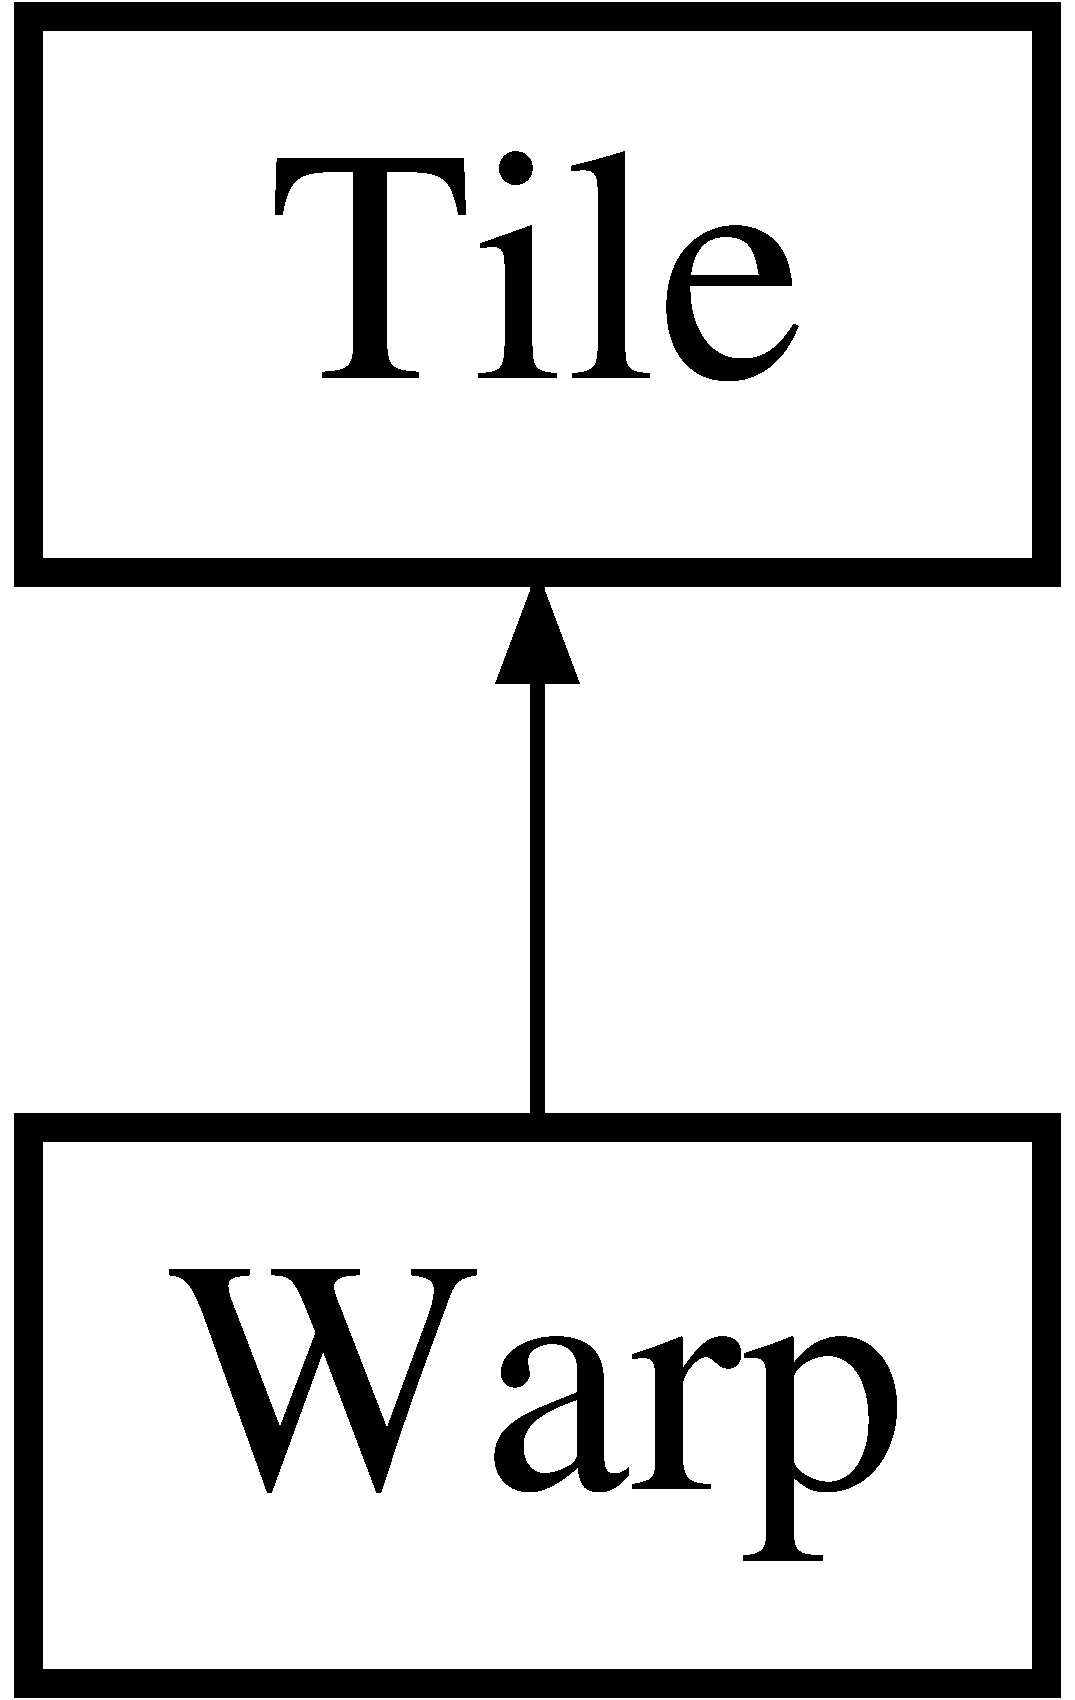
\includegraphics[height=2.000000cm]{class_tile}
\end{center}
\end{figure}
\subsection*{Public Member Functions}
\begin{DoxyCompactItemize}
\item 
\hyperlink{class_tile_ae8839483d411c1324a0c89327a557194}{Tile} (tile\+Type t=V\+O\+ID)\hypertarget{class_tile_ae8839483d411c1324a0c89327a557194}{}\label{class_tile_ae8839483d411c1324a0c89327a557194}

\begin{DoxyCompactList}\small\item\em \hyperlink{class_tile}{Tile} constructor. Makes a V\+O\+ID \hyperlink{class_tile}{Tile} by default. \end{DoxyCompactList}\item 
virtual \hyperlink{class_tile_a98634abbd93fa13d0578d7103202d03d}{$\sim$\+Tile} ()\hypertarget{class_tile_a98634abbd93fa13d0578d7103202d03d}{}\label{class_tile_a98634abbd93fa13d0578d7103202d03d}

\begin{DoxyCompactList}\small\item\em Virtual \hyperlink{class_tile}{Tile} destructor. \end{DoxyCompactList}\item 
void \hyperlink{class_tile_ab29acce6f4bf7ea4617213269e8c3716}{connect\+Tile} (dir d, \hyperlink{class_tile}{Tile} $\ast$t)\hypertarget{class_tile_ab29acce6f4bf7ea4617213269e8c3716}{}\label{class_tile_ab29acce6f4bf7ea4617213269e8c3716}

\begin{DoxyCompactList}\small\item\em Specifies an adjacent \hyperlink{class_tile}{Tile}. Not reciprocal -- may be one-\/way! \end{DoxyCompactList}\item 
virtual const string \hyperlink{class_tile_ae04dfcac010592c1ef0aaae031f31b6a}{enter\+Tile} ()
\item 
double \hyperlink{class_tile_a947b6692bfcdd7b1adc59fcbee16c1fc}{get\+Angle} ()\hypertarget{class_tile_a947b6692bfcdd7b1adc59fcbee16c1fc}{}\label{class_tile_a947b6692bfcdd7b1adc59fcbee16c1fc}

\begin{DoxyCompactList}\small\item\em Get the current angle of sprite rotation for the Tile’s art. \end{DoxyCompactList}\item 
S\+D\+L\+\_\+\+Renderer\+Flip \hyperlink{class_tile_ad2d2b3bd012d3a54ccb51f6eb986115a}{get\+Flip} ()\hypertarget{class_tile_ad2d2b3bd012d3a54ccb51f6eb986115a}{}\label{class_tile_ad2d2b3bd012d3a54ccb51f6eb986115a}

\begin{DoxyCompactList}\small\item\em Gets current flip status of Tile’s sprite. \end{DoxyCompactList}\item 
bool \hyperlink{class_tile_aaddc2d065a537489c31de4a566bb0bd5}{get\+Is\+Passable} ()\hypertarget{class_tile_aaddc2d065a537489c31de4a566bb0bd5}{}\label{class_tile_aaddc2d065a537489c31de4a566bb0bd5}

\begin{DoxyCompactList}\small\item\em Returns true if the \hyperlink{class_tile}{Tile} may be entered by a \hyperlink{class_unit}{Unit}. \end{DoxyCompactList}\item 
\hyperlink{class_tile}{Tile} $\ast$ \hyperlink{class_tile_ae5038e62f2a4c28150f6abb4deb31433}{get\+Tile} (dir d)\hypertarget{class_tile_ae5038e62f2a4c28150f6abb4deb31433}{}\label{class_tile_ae5038e62f2a4c28150f6abb4deb31433}

\begin{DoxyCompactList}\small\item\em Returns pointer to adjacent tile in specified direction. May be nullptr. \end{DoxyCompactList}\item 
tile\+Type \hyperlink{class_tile_a36871de25627c7483c31807da1c28706}{get\+Type} ()\hypertarget{class_tile_a36871de25627c7483c31807da1c28706}{}\label{class_tile_a36871de25627c7483c31807da1c28706}

\begin{DoxyCompactList}\small\item\em Returns the Tile’s type. \end{DoxyCompactList}\item 
int \hyperlink{class_tile_a25b90e07fd9cdaba1df3ac2a9b6d032b}{getX} ()\hypertarget{class_tile_a25b90e07fd9cdaba1df3ac2a9b6d032b}{}\label{class_tile_a25b90e07fd9cdaba1df3ac2a9b6d032b}

\begin{DoxyCompactList}\small\item\em Returns the Tile’s x position on its \hyperlink{class_terr}{Terr}. \end{DoxyCompactList}\item 
int \hyperlink{class_tile_acf97bff4aac74cc8d7e09bc8ca5afa68}{getY} ()\hypertarget{class_tile_acf97bff4aac74cc8d7e09bc8ca5afa68}{}\label{class_tile_acf97bff4aac74cc8d7e09bc8ca5afa68}

\begin{DoxyCompactList}\small\item\em Returns the Tile’s y position on its \hyperlink{class_terr}{Terr}. \end{DoxyCompactList}\item 
void \hyperlink{class_tile_a94f9e2d35e55c1d1b9f56dbd7816f51a}{set\+Angle} (double a)\hypertarget{class_tile_a94f9e2d35e55c1d1b9f56dbd7816f51a}{}\label{class_tile_a94f9e2d35e55c1d1b9f56dbd7816f51a}

\begin{DoxyCompactList}\small\item\em Sets the rotational angle of the Tile’s sprite. \end{DoxyCompactList}\item 
void \hyperlink{class_tile_a801a349b0e7f7500b60af91e5e821f2e}{set\+Flip} (S\+D\+L\+\_\+\+Renderer\+Flip f)\hypertarget{class_tile_a801a349b0e7f7500b60af91e5e821f2e}{}\label{class_tile_a801a349b0e7f7500b60af91e5e821f2e}

\begin{DoxyCompactList}\small\item\em Sets whether the Tile’s sprite is flipped. \end{DoxyCompactList}\item 
void \hyperlink{class_tile_a8a6429d2adbe3e45c519d86a57b514c3}{set\+Pos} (int x\+Pos, int y\+Pos)\hypertarget{class_tile_a8a6429d2adbe3e45c519d86a57b514c3}{}\label{class_tile_a8a6429d2adbe3e45c519d86a57b514c3}

\begin{DoxyCompactList}\small\item\em Sets where \hyperlink{class_tile}{Tile} thinks it is on a \hyperlink{class_terr}{Terr}. \end{DoxyCompactList}\item 
void \hyperlink{class_tile_a2557595d030a43cf9b5334df3b7264f7}{set\+Type} (tile\+Type t)\hypertarget{class_tile_a2557595d030a43cf9b5334df3b7264f7}{}\label{class_tile_a2557595d030a43cf9b5334df3b7264f7}

\begin{DoxyCompactList}\small\item\em Sets what kind of tile it is. \end{DoxyCompactList}\end{DoxyCompactItemize}
\subsection*{Protected Attributes}
\begin{DoxyCompactItemize}
\item 
int \hyperlink{class_tile_a47b5eb2072d4b1978923a480043899c9}{x}\hypertarget{class_tile_a47b5eb2072d4b1978923a480043899c9}{}\label{class_tile_a47b5eb2072d4b1978923a480043899c9}

\begin{DoxyCompactList}\small\item\em X-\/position \hyperlink{class_tile}{Tile} believes it holds on a \hyperlink{class_terr}{Terr}. \end{DoxyCompactList}\item 
int \hyperlink{class_tile_a2d87d8813151af6bbd60811964f047a8}{y}\hypertarget{class_tile_a2d87d8813151af6bbd60811964f047a8}{}\label{class_tile_a2d87d8813151af6bbd60811964f047a8}

\begin{DoxyCompactList}\small\item\em Y-\/position \hyperlink{class_tile}{Tile} believes it holds on a \hyperlink{class_terr}{Terr}. \end{DoxyCompactList}\item 
tile\+Type \hyperlink{class_tile_a5aa7ae6350675967edf46400c486a412}{type}\hypertarget{class_tile_a5aa7ae6350675967edf46400c486a412}{}\label{class_tile_a5aa7ae6350675967edf46400c486a412}

\begin{DoxyCompactList}\small\item\em Which type of tile to draw. \end{DoxyCompactList}\item 
bool \hyperlink{class_tile_afa72b458d549b9533f058e2d2fad0f81}{is\+Passable}
\item 
\hyperlink{class_tile}{Tile} $\ast$ \hyperlink{class_tile_a0d63c88d4136aecedcb2756d20615b89}{E}\hypertarget{class_tile_a0d63c88d4136aecedcb2756d20615b89}{}\label{class_tile_a0d63c88d4136aecedcb2756d20615b89}

\begin{DoxyCompactList}\small\item\em Adjacent \hyperlink{class_tile}{Tile} to the East/\+Right. \end{DoxyCompactList}\item 
\hyperlink{class_tile}{Tile} $\ast$ \hyperlink{class_tile_af1255bd2dba8dfa019fcd65a05805ed1}{N}\hypertarget{class_tile_af1255bd2dba8dfa019fcd65a05805ed1}{}\label{class_tile_af1255bd2dba8dfa019fcd65a05805ed1}

\begin{DoxyCompactList}\small\item\em Adjacent \hyperlink{class_tile}{Tile} to the North/\+Up. \end{DoxyCompactList}\item 
\hyperlink{class_tile}{Tile} $\ast$ \hyperlink{class_tile_adc655f39bc82d9b5898b991faea9df42}{S}\hypertarget{class_tile_adc655f39bc82d9b5898b991faea9df42}{}\label{class_tile_adc655f39bc82d9b5898b991faea9df42}

\begin{DoxyCompactList}\small\item\em Adjacent \hyperlink{class_tile}{Tile} to the South/\+Down. \end{DoxyCompactList}\item 
\hyperlink{class_tile}{Tile} $\ast$ \hyperlink{class_tile_ae992c1605ed059cb9eaff737b99824dc}{W}\hypertarget{class_tile_ae992c1605ed059cb9eaff737b99824dc}{}\label{class_tile_ae992c1605ed059cb9eaff737b99824dc}

\begin{DoxyCompactList}\small\item\em Adjacent \hyperlink{class_tile}{Tile} to the West/\+Left. \end{DoxyCompactList}\item 
double \hyperlink{class_tile_a33219999fbd38d9c9e8e98d09a9b65a5}{angle}\hypertarget{class_tile_a33219999fbd38d9c9e8e98d09a9b65a5}{}\label{class_tile_a33219999fbd38d9c9e8e98d09a9b65a5}

\begin{DoxyCompactList}\small\item\em Angle at which Tile’s sprite is rotated. \end{DoxyCompactList}\item 
S\+D\+L\+\_\+\+Renderer\+Flip \hyperlink{class_tile_a815af374aa83cd0be79bb5553056b15e}{flip}\hypertarget{class_tile_a815af374aa83cd0be79bb5553056b15e}{}\label{class_tile_a815af374aa83cd0be79bb5553056b15e}

\begin{DoxyCompactList}\small\item\em Flip status of Tile’s sprite. \end{DoxyCompactList}\end{DoxyCompactItemize}


\subsection{Detailed Description}
Data about individual tiles from a \hyperlink{class_terr}{Terr}. 

\subsection{Member Function Documentation}
\index{Tile@{Tile}!enter\+Tile@{enter\+Tile}}
\index{enter\+Tile@{enter\+Tile}!Tile@{Tile}}
\subsubsection[{\texorpdfstring{enter\+Tile()}{enterTile()}}]{\setlength{\rightskip}{0pt plus 5cm}const string Tile\+::enter\+Tile (
\begin{DoxyParamCaption}
{}
\end{DoxyParamCaption}
)\hspace{0.3cm}{\ttfamily [virtual]}}\hypertarget{class_tile_ae04dfcac010592c1ef0aaae031f31b6a}{}\label{class_tile_ae04dfcac010592c1ef0aaae031f31b6a}
Overridable base function for derived tiles doing something special when entered. Base functionality just sets \hyperlink{class_sprite}{Sprite}. 

Reimplemented in \hyperlink{class_warp_a28e607e491d761c1baad786e911a2681}{Warp}.



\subsection{Member Data Documentation}
\index{Tile@{Tile}!is\+Passable@{is\+Passable}}
\index{is\+Passable@{is\+Passable}!Tile@{Tile}}
\subsubsection[{\texorpdfstring{is\+Passable}{isPassable}}]{\setlength{\rightskip}{0pt plus 5cm}bool Tile\+::is\+Passable\hspace{0.3cm}{\ttfamily [protected]}}\hypertarget{class_tile_afa72b458d549b9533f058e2d2fad0f81}{}\label{class_tile_afa72b458d549b9533f058e2d2fad0f81}
True if tile can be entered. May change later to enterable from each side. 

The documentation for this class was generated from the following files\+:\begin{DoxyCompactItemize}
\item 
Tile.\+h\item 
Tile.\+cpp\end{DoxyCompactItemize}

\hypertarget{class_unit}{}\section{Unit Class Reference}
\label{class_unit}\index{Unit@{Unit}}


Backend of a character’s data. Visual depiction handled by \hyperlink{class_sprite}{Sprite} class.  




{\ttfamily \#include $<$Unit.\+h$>$}



\subsection{Detailed Description}
Backend of a character’s data. Visual depiction handled by \hyperlink{class_sprite}{Sprite} class. 

The documentation for this class was generated from the following file\+:\begin{DoxyCompactItemize}
\item 
Unit.\+h\end{DoxyCompactItemize}

\hypertarget{class_warp}{}\section{Warp Class Reference}
\label{class_warp}\index{Warp@{Warp}}


\hyperlink{class_warp}{Warp} is a kind of \hyperlink{class_tile}{Tile} that loads a new \hyperlink{class_terr}{Terr} (e.\+g. leaving a building).  




{\ttfamily \#include $<$Warp.\+h$>$}

Inheritance diagram for Warp\+:\begin{figure}[H]
\begin{center}
\leavevmode
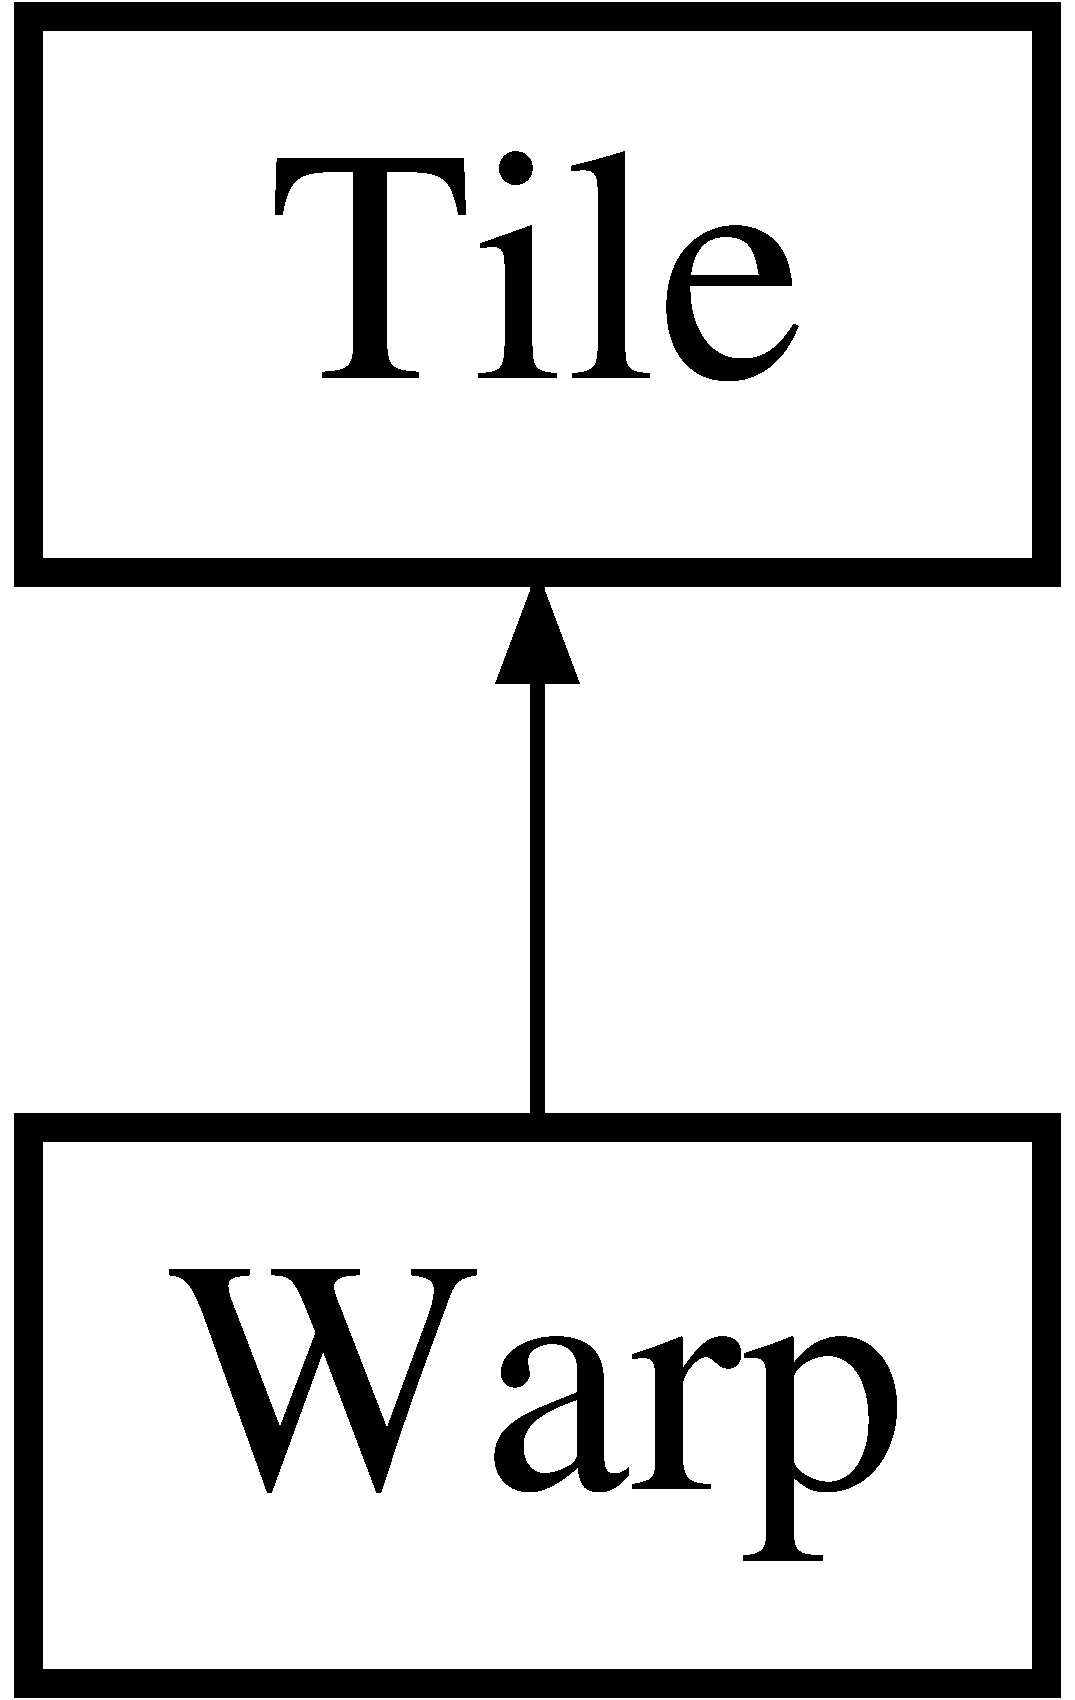
\includegraphics[height=2.000000cm]{class_warp}
\end{center}
\end{figure}
\subsection*{Protected Attributes}
\begin{DoxyCompactItemize}
\item 
string \hyperlink{class_warp_abbc0edf4c6a9939e0c39c9eb55b8fb1f}{new\+Terr}\hypertarget{class_warp_abbc0edf4c6a9939e0c39c9eb55b8fb1f}{}\label{class_warp_abbc0edf4c6a9939e0c39c9eb55b8fb1f}

\begin{DoxyCompactList}\small\item\em filename of new \hyperlink{class_terr}{Terr} \end{DoxyCompactList}\end{DoxyCompactItemize}
\subsection*{Additional Inherited Members}


\subsection{Detailed Description}
\hyperlink{class_warp}{Warp} is a kind of \hyperlink{class_tile}{Tile} that loads a new \hyperlink{class_terr}{Terr} (e.\+g. leaving a building). 

The documentation for this class was generated from the following file\+:\begin{DoxyCompactItemize}
\item 
Warp.\+h\end{DoxyCompactItemize}

%--- End generated contents ---

% Index
\backmatter
\newpage
\phantomsection
\clearemptydoublepage
\addcontentsline{toc}{chapter}{Index}
\printindex

\end{document}
